\section{COVID-19 AND DRONE}
\label{covid19section}
\textcolor{red}{
The novel coronavirus, known as COVID-19 has emerged as a global pandemic in 2020 and ravaged the social and economic life of the people across the globe. The ubiquitous nature of drones has proven aptly helpful in a number of use cases, from performing COVID-19 related risk assessment, monitoring to providing real-time support to citizens and authorities in a number of countries. Despite the increase in such specialized use cases, the drone industry has suffered from continued financial losses due to lower consumer space demand and reduced manufacturing capacity as a result of factory shutdowns. In this section, we briefly discuss the details of these circumstances.}
% Like other organizations, the drone industry has also suffered financial losses. 
% On the other hand, these drones helped us a lot to tackle this situation in several ways. 
% All of these will be discussed below. 
% A metaphorical picture is portrayed in Fig~\ref{dronevscovid}.
% \begin{figure}[h!]
% \centering
% 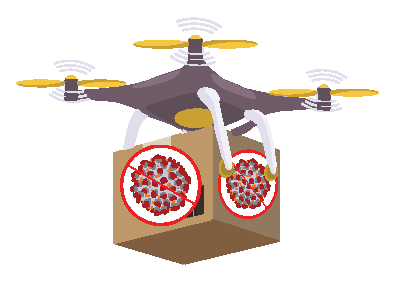
\includegraphics[width=.5\linewidth]{figure/dronevscovid.eps}
% \caption{A metaphorical picture of drone vs COVID-19.}
% \label{dronevscovid}
% \end{figure}

\subsection{Usage of Drone in COVID-19 Situation}
% The most prospective use of a drone can be possible during a pandemic situation~\cite{dronecnn}
\textcolor{red}{
The autonomous operation capabilities of drones, paired with visual and audio sensing modalities provide them with unparalleled flexibility in contactless monitoring and delivery operations. Indeed, during COVID-19 crisis, 
}
% During COVID-19, contactless delivery and autonomous vehicles are badly needed to help keep people out of risk. A drone has not only autonomous operation capabilities but also vision and hearing senses, which can monitor surroundings.
% Therefore, 
\textcolor{red}{
several countries utilized drones to carry supplies and warn their citizens. For example, during the initial stage of the pandemic, China used drones to encourage citizens to wear protective gears and masks. [CITE]
In Indonesia, United Arab Emirates and Spain, drones were commissioned to deploy disinfectants in areas deemed too dangerous for humans [CITE].
In Saudi Arabia and Italy, authorities have been using the thermal drone to pre-screen abnormal body temperatures. 
}
% Although drones can not measure the temperature of the body precisely, they can distinguish people with abnormal body temperatures corresponding to the surroundings. 
In Chile, authorities have been using drones to distribute drugs to people in remote rural areas. Like other nations, drones are also being used in the United States during the pandemic~\cite{dronefortune}. In Grand Forks, North Dakota, local Walmarts are offering new home delivery options of food and medical supplies by drones. Some companies are interested in utilizing drones to fight the virus, e.g., spraying disinfectants in large, or searching infected people in the crowds using the thermal vision of the drone.

\subsection{Effects of COVID-19 on Drone Industry}
A very challenging decade for drone industry has started in the year of 2020. A chart of the predicted industry value of drone in 2021 is shown in Fig~\ref{dronemarket}.
\begin{figure}[h!]
\centering

\includegraphics[width=.8\linewidth]{figure/dronemarket.eps}
\caption{Predicted market value of different sectors.}
\label{dronemarket}
\end{figure}
According to the Business Insider source~\cite{dronebusinessinsider}, the expected drone sale in 2021 will surpass 12 billion dollars, increased by 7.6\%  annual growth rate (CAGR) compared to 2016, when the sale was 8.5 billion dollars. %(parle CAGR graph: https://www.businessinsider.com/uav-or-commercial-drone-market-forecast-2016-4-28).
The major contribution will come from three sectors. Consumer drone sales are forecast to reach 29 million, whereas commercial shipments of drones are expected to exceed .8 billion dollars. 
%(maybe top producer of drone company)

All the predictions mentioned above are before the COVID-19 situation. Like other industrial sectors, this pandemic situation has affected the drone industry a lot. A large number of electrical component manufacturers are facing stability problems or shutdowns, as the virus affects the production line workers. As a result, worldwide drone companies are failing to reach production deadlines. In 2020, the United States accounts for more than 29\% of global drone market share, and China holds around 16\% of the global share. Following the coronavirus outbreak in January 2019, China's exports have decreased substantially. As a result, significant casualties happened to the drone industries that are reliant on the trade of batteries, cameras, or other components manufactured from China. Though the United States-based companies are ensembling drones, they are also struggling from the supply-chain disturbance. Nevertheless, according to the Forbes news, the demand, and revenue of the global drone industry will experience a quick recovery in the upcoming year~\cite{droneforbes}. The prediction about the drone market worldwide after the pandemic is to reach 77.5 billion dollars by the end of 2027~\cite{droneglobenewswire}. Predicted sales of drone after and before COVID-19 situation is shown in Fig~\ref{dronesale}.
\begin{figure}[h!]
\centering
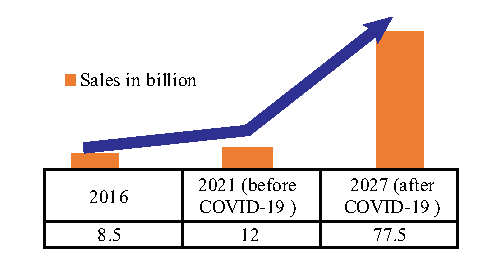
\includegraphics[width=.8\linewidth]{figure/dronesale.eps}
\caption{Predicted sales of drone after and before COVID-19 situation.}
\label{dronesale}
\end{figure}